\chapter{SPEXS Generalization}
\label{c:generalization}

In this chapter we show how to make SPEXS algorithm more abstract by allowing flexibilty through function composition and finding minimal requirements for the data-structures.

\section{Algorithm}

The algorithm in a more conventional view is:

\begin{algorithm}[H]
	\caption{The spexs2 algorithm}
\begin{algorithmic}[1]
	\Require{$dataset$, $in$ and $out$ are pools, $extend$ is an extender function, $extend?$, $output?$ are filters}
	\Ensure{Patterns satisfying filters and $extender$ are in $out$ pool}
	\Statex
	\Function{spexs2}{dataset, in, out, extend, extend?, output?}
		\State prepare(in, dataset)
		\While{$q \gets $ in.pop()}
			\Let{extended}{extend($q$, dataset)}
			\For{ $qx \in $ extended }
				\If{ extend?($qx$) }
					\State in.push($qx$)
					\If{ output?($qx$) }
						\State out.push($qx$)
					\EndIf
				\EndIf
			\EndFor
		\EndWhile
	\EndFunction
\end{algorithmic}
\end{algorithm}

When the algorithm starts by initializing the \emph{in} pool. The \emph{in} pool shall contain queries which we wish to further examine. In the simplest case this means we create an empty pattern query and put it into the \emph{in} pool. We could also start the process with an already existing pattern.

As the next step we pick a query from the \emph{in} pool for extending. The extending means generating all queries whose pattern size is larger by one. There can be several such queries.

If any of the queries should be further examined as defined by the \emph{extendable} query filter, it will be put into the \emph{in} pool.

If the query is suitable for output as defined by the \emph{outputtable} filter, it will be put into the \emph{out} pool. 

If we extend each pattern at each step by one we guarantee that we examine all the patterns that conform to our criteria as defined by \emph{extendable} filter.

\section{Pools}

Since pools act independently from the rest of the algorithm they are free to reorder, store on disk or even discard the queries, if needed. If we wish to get 100 best results the output pool could immediately discard the bad ones.

We can also use different types of structures as pools. For example using a queue would make it start examining breadth first, using a stack would make it run depth first. We can use priority queue to choose the best queries to reach faster the good results as suggested in "Patterns Discovery from Biosequences"\cite{spexs}.

\section{Filtering}

Filtering allows us to reduce the number of queries we have to examine and allows to select a subset of queries by some criteria.

The filters can make the decision, whether the query should be extended, based on any available information. For example query pattern, number of occurences, metadata in sequences, metadata in dataset or use data from configuration.

\begin{exmp}
We can add metadata to the sequence about the datafile. We count the occurences of a query in each datafile and then if the ratio between counts is smaller than some number defined in the configuration.
\end{exmp}

Although there is only one filter "function" specified the filter could be a composite of multiple filters.

\begin{exmp}
Pattern length is greater than three and pattern occurs at least 10 times in the dataset can be seen as a single filter that is composed of two filters.
\end{exmp}

\section{Extending}

The extending process is at the core of the algorithm and there are several ways of doing it. The main criteria is that the extending should guarantee that all possible patterns get eventually enumerated.

Extender is analogous to an inductive step. Our base case is formulated by \emph{prepare} step in the SPEXS2 algorithm and the induction steps are carried out by the extender.

\begin{exmp}
We start with an empty query and we know all the locations of it. If our extender generates all the queries where the patterns are longer by 1 then we are guaranteed to enumarate all the patterns.
\end{exmp}

\begin{exmp}
We can start with the empty query and all queries with patterns of length 1. Now if our extender generates queries where the patterns are longer by 2 we can also examine all of the queries.
\end{exmp}

The extender determines which patterns and pattern classes will be generated. We can modify and compose different extenders to get new patterns. Often more complex patterns can adversely affect performance.

The general idea for extending is to find all the following patterns from all the previous query positions and then group the similar patterns into queries.

This process can be visualized with graphs. We make the sequence into a graph where the links between nodes are the sequence tokens. Each pattern then can walk the edges and match find the ending position for each pattern.

For example the sequence \R{ACGCCGATCGC} would look like:

\begin{figure}[H]
	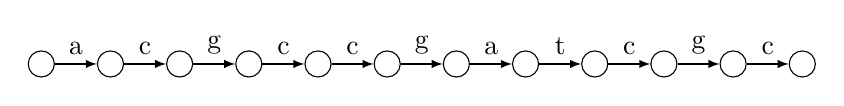
\begin{tikzpicture}[auto]
	\tikzstyle{state} = [ draw, circle, thin, node distance = 2.5em, font={\small}];
	\tikzstyle{query} = [ draw, rectangle, thin, node distance = 2.5em, font={\small}];
	\tikzstyle{info} = [font={\itshape\footnotesize}]
	\tikzstyle{point}  = [ ->, thin, font={\small}];
	\tikzstyle{extend} = [ ->, double, font={\small}];
	\tikzstyle{trace} = [ ->, thick, dashed, bend right, font={\small} ];

	\def \seq {x,a,c,g,c,c,g,a,t,c,g,c}

	\foreach \x [count=\xi] in \seq {
		\ifnum 1 < \xi
			\pgfmathparse{int(\xi-1)}
			\let \li \pgfmathresult
			\node[state, right of=\li] (\xi) {};
			\draw[->, >=latex] (\li) to node{\x} (\xi);
		\else
			\node[state] (\xi) {};
		\fi
	}
\end{tikzpicture}

\end{figure}

For simplicity we use nucleotides as our alphabet $\Sigma = \{ \R{A}, \R{C}, \R{G}, \R{T} \}$ in the following examples.

\subsection{Sequences}

The simplest case how the \emph{next} function behaves is when we are only looking for simple sequences. Let's consider a sequence \R{ACGCCGATCGC} and a pattern \R{CG}.

\begin{figure}[H]
	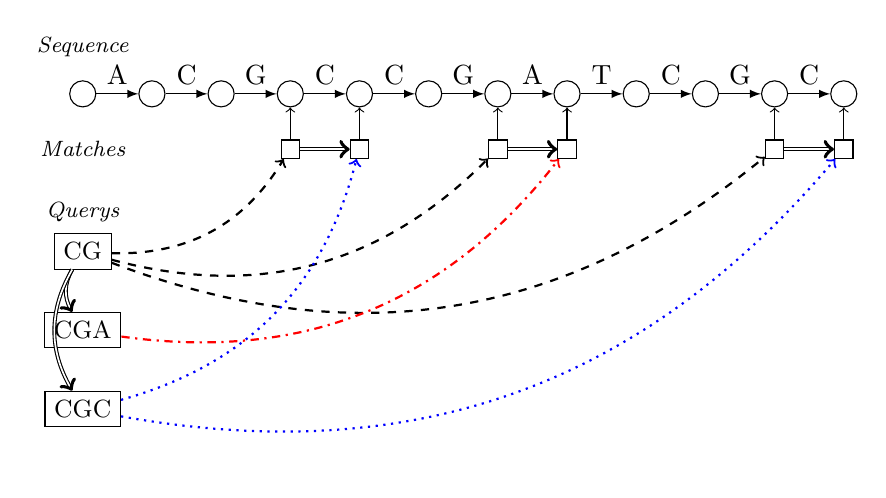
\begin{tikzpicture}[auto]
	\tikzstyle{state} = [ draw, circle, thin, node distance = 2.5em, font={\small}];
	\tikzstyle{query} = [ draw, rectangle, thin, node distance = 2.5em, font={\small}];
	\tikzstyle{info} = [font={\itshape\footnotesize}]
	\tikzstyle{point}  = [ ->, thin, font={\small}];
	\tikzstyle{extend} = [ ->, double, font={\small}];
	\tikzstyle{trace} = [ ->, thick, dashed, bend right, font={\small} ];

	\def \seq {X,A,C,G,C,C,G,A,T,C,G,C}

	\foreach \x [count=\xi] in \seq {
		\ifnum 1 < \xi
			\pgfmathparse{int(\xi-1)}
			\let \li \pgfmathresult
			\node[state, right of=\li] (\xi) {};
			\draw[->, >=latex] (\li) to node{\x} (\xi);
		\else
			\node[state] (\xi) {};
		\fi
	}

	\node[info] at (0,0.6) {Sequence};
	\node[info] at (0,-0.7) {Matches};
	\node[info] at (0,-1.5) {Querys};

	\node[query](CG)  at (0,-2) {CG};
	\node[query](CGA) at (0,-3) {CGA};
	\node[query](CGC) at (0,-4) {CGC};

	\tikzstyle{traceCG} = [ ->, thick, dashed, bend right, color=black ];
	\tikzstyle{traceCGA} = [ ->, thick, dashdotted, bend right, color=red ];
	\tikzstyle{traceCGC} = [ ->, thick, dotted, bend right, color=blue ];

	\draw[extend, bend right] (CG) to (CGA);
	\draw[extend, bend right] (CG) to (CGC);

	\foreach \xi/\xv in {4/CG,7/CG,11/CG} {
		\node[draw, below of=\xi, node distance=2em] (p\xi) {};
		\draw[point] (p\xi) to (\xi);
		\draw[trace\xv] (\xv) to (p\xi);
	}

	\foreach \xi/\xv in {5/CGC,8/CGA,12/CGC} {
		\node[draw, below of=\xi, node distance=2em] (p\xi) {};
		\draw[point] (p\xi) to (\xi);
		\draw[trace\xv] (\xv) to (p\xi);
	}

	\foreach \xi/\yi in {4/5,7/8,11/12} {
		\draw[extend] (p\xi) to (p\yi);
	}
\end{tikzpicture}

\end{figure}

Initially we have matches only for query \R{CG}. Then by taking the \emph{next} token from the sequence we can build up querys \R{CGA} and \R{CGC}.

\subsection{Group tokens}

One common addition in a pattern language is matching a group of tokens. For example we can use $\R{X} = \R{[AC]}$ to denote both tokens \R{A}, \R{C}. By adding where either one transitions we can capture such groups in the extension process.

\begin{figure}[H]
	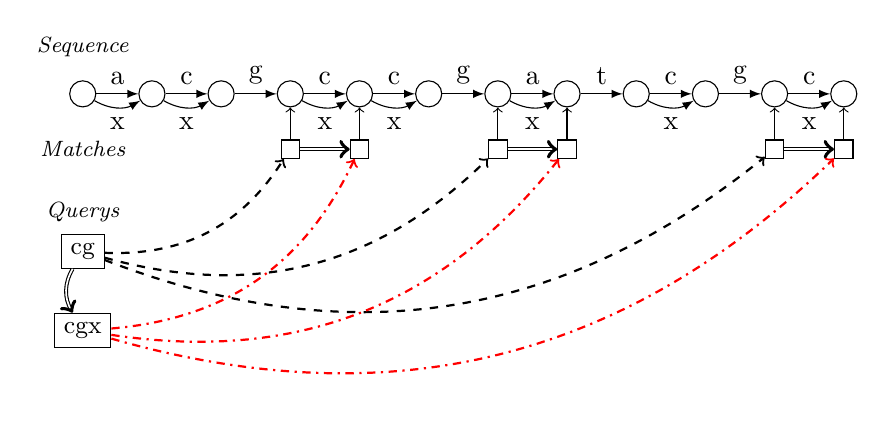
\begin{tikzpicture}[auto]
	\tikzstyle{state} = [ draw, circle, thin, node distance = 2.5em, font={\small}];
	\tikzstyle{query} = [ draw, rectangle, thin, node distance = 2.5em, font={\small}];
	\tikzstyle{info} = [font={\itshape\footnotesize}]
	\tikzstyle{point}  = [ ->, thin, font={\small}];
	\tikzstyle{extend} = [ ->, double, font={\small}];
	\tikzstyle{trace} = [ ->, thick, dashed, bend right, font={\small} ];

	\def \seq {x,a,c,g,c,c,g,a,t,c,g,c}

	\foreach \x [count=\xi] in \seq {
		\ifnum 1 < \xi
			\pgfmathparse{int(\xi-1)}
			\let \li \pgfmathresult
			\node[state, right of=\li] (\xi) {};
			\draw[->, >=latex] (\li) to node{\x} (\xi);
		\else
			\node[state] (\xi) {};
		\fi
	}

	\tikzstyle{exstate} = [ ->, bend right, >=latex];
	\foreach \xi/\yi in {1/2,2/3,4/5,5/6,7/8,9/10,11/12} {
		\draw[exstate] (\xi) to node[below]{x} (\yi);
	}


	\node[info] at (0,0.6) {Sequence};
	\node[info] at (0,-0.7) {Matches};
	\node[info] at (0,-1.5) {Querys};

	\node[query](cg)  at (0,-2) {cg};
	\node[query](cgx) at (0,-3) {cgx};

	\tikzstyle{tracecg} = [ ->, thick, dashed, bend right, color=black ];
	\tikzstyle{tracecgx} = [ ->, thick, dashdotted, bend right, color=red ];

	\draw[extend, bend right] (cg) to (cgx);

	\foreach \xi/\xv in {4/cg,7/cg,11/cg} {
		\node[draw, below of=\xi, node distance=2em] (p\xi) {};
		\draw[point] (p\xi) to (\xi);
		\draw[trace\xv] (\xv) to (p\xi);
	}

	\foreach \xi/\xv in {5/cgx,8/cgx,12/cgx} {
		\node[draw, below of=\xi, node distance=2em] (p\xi) {};
		\draw[point] (p\xi) to (\xi);
		\draw[trace\xv] (\xv) to (p\xi);
	}

	\foreach \xi/\yi in {4/5,7/8,11/12} {
		\draw[extend] (p\xi) to (p\yi);
	}
\end{tikzpicture}

\end{figure}

There is a universal group \R{.} or \emph{wildcard} that matches any token in the alphabet.

\begin{exmp}
Pattern \R{T.} would match patterns \R{TA}, \R{TC}, \R{TG}, \R{TT}.
\end{exmp}

\subsection{Star}

Another possible extension is capturing a run of wildcards.

\begin{exmp}
A pattern \R{A.*T} would match \R{ACT}, \R{ATTC}, \R{ATTTC} and so on.
\end{exmp}

On the graph instead of \R{.*} we use only \R{*} symbol.

\begin{figure}[H]
	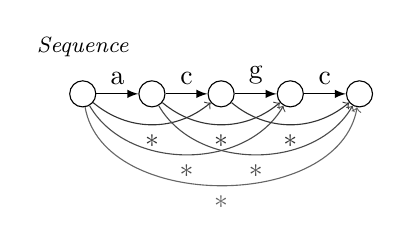
\begin{tikzpicture}[auto]
	\tikzstyle{state} = [ draw, circle, thin, node distance = 2.5em, font={\small}];
	\tikzstyle{query} = [ draw, rectangle, thin, node distance = 2.5em, font={\small}];
	\tikzstyle{info} = [font={\itshape\footnotesize}]
	\tikzstyle{point}  = [ ->, thin, font={\small}];
	\tikzstyle{extend} = [ ->, double, font={\small}];
	\tikzstyle{trace} = [ ->, thick, dashed, bend right, font={\small} ];

	\def \seq {x,a,c,g,c}

	\foreach \x [count=\xi] in \seq {
		\ifnum 1 < \xi
			\pgfmathparse{int(\xi-1)}
			\let \li \pgfmathresult
			\node[state, right of=\li] (\xi) {};
			\draw[->, >=latex] (\li) to node{\x} (\xi);
		\else
			\node[state] (\xi) {};
		\fi
	}

	\node[info] at (0,0.6) {Sequence};

	\tikzstyle{star} = [ ->, bend right, thin, color=black ];

	\foreach \xi in {1,...,3} {
		\pgfmathparse{int(\xi+2)}
		\let \xinext \pgfmathresult
		\foreach \yi in {\xinext,...,5} {
			\pgfmathparse{int(\yi - \xi)}
			\let \df \pgfmathresult
			\pgfmathparse{-\df*20}
			\let \out \pgfmathresult
			\pgfmathparse{int(180 - \out)}
			\let \in \pgfmathresult
			\pgfmathparse{int(100-\df*10)}
			\let \shade \pgfmathresult
			\draw[star, out=\out, in=\in, color=black!\shade] (\xi) to node[below]{$*$} (\yi);
		}
	}

\end{tikzpicture}

\end{figure}

Constructing more complicated patterns increases the amount of queries required to enumerate. There are of course optimizations to avoid intermediary steps and repeated walking on the dataset. For example we can skip the extension with only \R{.*} and instead extend with \R{.*Y}, where \R{Y} is a token from the alphabet. This means we avoid this one large query and instead have multiple smaller queries.

\begin{figure}[H]
	\begin{tikzpicture}[auto]
	\tikzstyle{state} = [ draw, circle, thin, node distance = 2.5em, font={\small}];
	\tikzstyle{query} = [ draw, rectangle, thin, node distance = 2.5em, font={\small}];
	\tikzstyle{info} = [font={\itshape\footnotesize}]
	\tikzstyle{point}  = [ ->, thin, font={\small}];
	\tikzstyle{extend} = [ ->, double, font={\small}];
	\tikzstyle{trace} = [ ->, thick, dashed, bend right, font={\small} ];


	\def \seq {X,A,C,G,C}

	\foreach \x [count=\xi] in \seq {
		\ifnum 1 < \xi
			\pgfmathparse{int(\xi-1)}
			\let \li \pgfmathresult
			\node[state, right of=\li] (\xi) {};
			\draw[->, >=latex] (\li) to node{\x} (\xi);
		\else
			\node[state] (\xi) {};
		\fi
	}

	\node[info] at (0,0.6) {Sequence};

	\tikzstyle{starC} = [ ->, bend right, thin, color=red ];
    \tikzstyle{starG} = [ ->, bend right, thin, color=blue ];

	\foreach \xi in {1,...,3} {
        \foreach \y [count=\yi] in \seq {
            \ifnumless{\xi+1}{\yi}{
                \pgfmathparse{int(\yi - \xi)}
                \let \df \pgfmathresult
                \pgfmathparse{-\df*20}
                \let \out \pgfmathresult
                \pgfmathparse{int(180 - \out)}
                \let \in \pgfmathresult

                \let \pat \seq[3]
                \draw[star\y, out=\out, in=\in] (\xi) to node[below]{$*$\y} (\yi);
            }
        }
	}

\end{tikzpicture}

\end{figure}

We can limit the length of the run to speed up the process. Limiting the run length to be either 2 or 3 would look like:

\begin{figure}[H]
	\begin{tikzpicture}[auto]
	\tikzstyle{state} = [ draw, circle, thin, node distance = 2.5em, font={\small}];
	\tikzstyle{query} = [ draw, rectangle, thin, node distance = 2.5em, font={\small}];
	\tikzstyle{info} = [font={\itshape\footnotesize}]
	\tikzstyle{point}  = [ ->, thin, font={\small}];
	\tikzstyle{extend} = [ ->, double, font={\small}];
	\tikzstyle{trace} = [ ->, thick, dashed, bend right, font={\small} ];


	\def \seq {X,A,C,G,C,C,G,A,T,C,G,C}

	\foreach \x [count=\xi] in \seq {
		\ifnum 1 < \xi
			\pgfmathparse{int(\xi-1)}
			\let \li \pgfmathresult
			\node[state, right of=\li] (\xi) {};
			\draw[->, >=latex] (\li) to node{\x} (\xi);
		\else
			\node[state] (\xi) {};
		\fi
	}

	\node[info] at (0,0.6) {Sequence};

	\tikzstyle{starC} = [ ->, bend right, thin, color=red ];
    \tikzstyle{starG} = [ ->, bend right, thin, color=blue ];
    \tikzstyle{starA} = [ ->, bend right, thin, color=green ];
    \tikzstyle{starT} = [ ->, bend right, thin, color=black ];

	\foreach \x [count=\xi] in \seq {
        \foreach \y [count=\yi] in \seq {
        	\pgfmathparse{int(\yi - \xi)}
            \let \df \pgfmathresult

            \ifnumcomp{1}{<}{\df}{
               	\ifnumcomp{\df}{<}{4}{
                	\pgfmathparse{-\df*20}
	                \let \out \pgfmathresult
	                \pgfmathparse{int(180 - \out)}
	                \let \in \pgfmathresult

	                \let \pat \seq[3]
	                \draw[star\y, out=\out, in=\in] (\xi) to node[below]{$*$\y} (\yi);
                }{}
            }{}
        }
	}

\end{tikzpicture}

\end{figure}

\subsection{Optimized group tokens}

Instead of immediately extending the group tokens we can take the output of an other extender and combine its results. If we have a group token $\gamma$ that contains $tokens(\gamma)$ then the \emph{matches} for such group is $$matches(p\gamma, D) = \bigcup_{t \in tokens(\gamma)} matches(pt, D) $$.

\begin{exmp}
A pattern \R{A[CTG]} is located in document $D$ at positions $matches(\R{AC}, D) + matches(\R{AT}, D) + matches(\R{AG}, D)$.
\end{exmp}

\subsection{Other possible extensions}

By adding a multi-step from a node to itself and to the next node we can capture optional tokens.

\begin{exmp}
A optional token \R{Y?} means that the token \R{Y} can occur either zero or one time. For example \R{AT?} matches \R{A} and \R{AT}.
\end{exmp}

The graph for such token would look like:

\begin{figure}[H]
	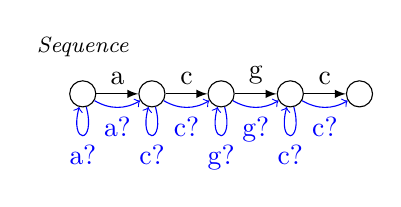
\begin{tikzpicture}[auto]
	\tikzstyle{state} = [ draw, circle, thin, node distance = 2.5em, font={\small}];
	\tikzstyle{query} = [ draw, rectangle, thin, node distance = 2.5em, font={\small}];
	\tikzstyle{info} = [font={\itshape\footnotesize}]
	\tikzstyle{point}  = [ ->, thin, font={\small}];
	\tikzstyle{extend} = [ ->, double, font={\small}];
	\tikzstyle{trace} = [ ->, thick, dashed, bend right, font={\small} ];


	\def \seq {x, a, c, g, c}

	\foreach \x [count=\xi] in \seq {
		\ifnum 1 < \xi
			\pgfmathparse{int(\xi-1)}
			\let \li \pgfmathresult
			\node[state, right of=\li] (\xi) {};
			\draw[->, >=latex] (\li) to node{\x} (\xi);
		\else
			\node[state] (\xi) {};
		\fi
	}

	\node[info] at (0,0.6) {Sequence};

    \tikzstyle{starQ} = [->, thin, color=blue ];

	\foreach \x [count=\xi] in \seq {
		\ifnum 1 < \xi
			\pgfmathparse{int(\xi-1)}
			\let \li \pgfmathresult
			\draw[starQ, bend right] (\li) to node[below]{\x?} (\xi);
			\draw[starQ, loop below] (\li) to node{\x?} (\li);
		\else
		\fi
	}
\end{tikzpicture}

\end{figure}

 Similarly we can use the same technique for optimization as for the group tokens ($matches(pY, D) = matches(p) \cup matches(pY)$, where $Y$ is a token).

\subsection{Alternative extensions}

We mentioned that we can also extend by different number of tokens at a time as long as we guarantee that all patterns will be searched. For optimality we also do not want to iterate over the same pattern multiple times. As a simple example the sequence \R{ACGCGA} could be iterated with setup:

\begin{figure}[H]
	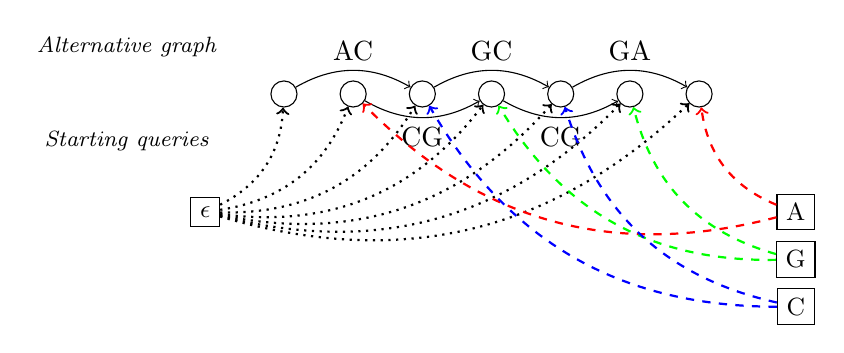
\begin{tikzpicture}[auto]
	\tikzstyle{state} = [ draw, circle, thin, node distance = 2.5em, font={\small}];
	\tikzstyle{query} = [ draw, rectangle, thin, node distance = 2.5em, font={\small}];
	\tikzstyle{info} = [font={\itshape\footnotesize}]
	\tikzstyle{point}  = [ ->, thin, font={\small}];
	\tikzstyle{extend} = [ ->, double, font={\small}];
	\tikzstyle{trace} = [ ->, thick, dashed, bend right, font={\small} ];


	\def \seq {X, A, C, G, C, G, A}

	\foreach \x [count=\xi] in \seq {
		\ifnum 1 < \xi
			\pgfmathparse{int(\xi-1)}
			\let \li \pgfmathresult
			\node[state, right of=\li] (\xi) {};
		\else
			\node[state] at(2,0) (\xi) {};
		\fi
	}

	\tikzstyle{labove} = [->, thin, bend left];
	\tikzstyle{lbelow} = [->, thin, bend right];

	\draw[labove] (1) to node[above]{AC} (3);
	\draw[lbelow] (2) to node[below]{CG} (4);
	\draw[labove] (3) to node[above]{GC} (5);
	\draw[lbelow] (4) to node[below]{CG} (6);
	\draw[labove] (5) to node[above]{GA} (7);

	\node[info] at (0,0.6) {Alternative graph};
	\node[info] at (0,-0.6) {Starting queries};

	\node[query](x) at (1,-1.5) {$\epsilon$};
	\node[query](A) at (8.5,-1.5) {A};
	\node[query](C) at (8.5,-2.7) {C};
	\node[query](G) at (8.5,-2.1) {G};

	\tikzstyle{tx} = [ ->, thick, dotted, bend right, color=black ];
	\tikzstyle{ta} = [ ->, thick, dashed, bend left, color=red ];
	\tikzstyle{tc} = [ ->, thick, dashed, bend left, color=blue ];
	\tikzstyle{tg} = [ ->, thick, dashed, bend left, color=green ];

	\draw[tx] (x) to (1);
	\draw[tx] (x) to (2);
	\draw[tx] (x) to (3);
	\draw[tx] (x) to (4);
	\draw[tx] (x) to (5);
	\draw[tx] (x) to (6);
	\draw[tx] (x) to (7);

	\draw[ta] (A) to (2);
	\draw[tc] (C) to (3);
	\draw[tg] (G) to (4);
	\draw[tc] (C) to (5);
	\draw[tg] (G) to (6);
	\draw[ta] (A) to (7);
\end{tikzpicture}

\end{figure}

Since at the starting point we have all the patterns of length 0 and 1, by adding patterns with length 2 we can be sure to enumerate all of them. Of course the previous methods for group and star patterns require modification.

\section{Summary}

The extender was shown to work via graphs, practically it is much more reasonable to minimize it as simple sequence as already mentioned in "Pattern Discovery from Biosequences"\cite{spexs}. The additional extension links shown in the graphs can either be precalculated or calculated at runtime.

From the previous results we can also derive the minimal requirements for the dataset. First we need to get the initial empty query - which means we should be somehow be able to get all the positions where a pattern could start. The other operator is finding the next position and token from a given position. Finding of next positions from a given positions on sequence can be interpreted as a forward iterator.

Since the best way to visualize was on graphs suggests that the \emph{spexs2} algorithm could be made to work on trees and then on graphs. Finding sequential patterns from a tree should be straightforward since the generic algorithm is oblivious to the amount of following tokens any position can have. Graphs can be more difficult since we need to remove duplicates caused by other extensions.

To use this generic version of the SPEXS algorithm we need to 1. choose our pool structures, 2. choose our filters, 3. choose our extender and preparation and 4. dataset implementation.
